\documentclass[12pt]{article}

	\usepackage{lmodern}
\usepackage{amssymb}
\usepackage{graphicx}
\usepackage{amsmath}
\usepackage{multirow}
\usepackage{mathtools}
\usepackage{placeins}
\usepackage{lscape}
\usepackage{geometry}
\usepackage{dcolumn}
\usepackage[utf8]{inputenc}
\usepackage{hyperref}
\usepackage{tabularx}
\usepackage{nicematrix}
\usepackage{calc}
\usepackage{qtree}
\usepackage{tikz}
\usepackage{setspace}
\usepackage[utf8]{inputenc}

	
	\usepackage{fullpage} %sets 1-in margins
	\newcommand{\tab}{\hspace*{2em}} %creates a \tab command, gives you horizontal space

	\setlength\parindent{0em} %sets indent
	 %\pagestyle{empty} %turns off page numbering on all pages

\makeatletter
\setlength{\@fptop}{0pt}
\setlength{\@fpbot}{0pt plus 1fil}
\makeatother

\title{SOFR and Crowding-Out Effect}
\date{\today}
\author{Qian Wu}

\begin{document}

\maketitle

\section{Empirical Findings}
\subsection{Response of SOFR and LIBOR to Gov't Borrowing}
\begin{center}
\footnotesize
\begin{tabular}{@{\extracolsep{5pt}}lD{.}{.}{-3} D{.}{.}{-3} D{.}{.}{-3} D{.}{.}{-3} } 
\\[-1.8ex]\hline 
\hline \\[-1.8ex] 
\multicolumn{5}{c}{\textit{Panel A: Gov't debt outstanding as the measure of borrowing}} \\ 
\cline{1-5} \\
 & \multicolumn{4}{c}{\textit{Dependent variable:}} \\ 
 \cline{2-5} \\
\\[-1.8ex] & \multicolumn{2}{c}{SOFR} & \multicolumn{2}{c}{LIBOR} \\ 
\\[-1.8ex] & \multicolumn{1}{c}{(1)} & \multicolumn{1}{c}{(2)} & \multicolumn{1}{c}{(3)} & \multicolumn{1}{c}{(4)}\\ 
\hline \\[-1.8ex] 
$\Delta$log debt & 386.758^{***} & 381.218^{***} & -34.675^{**} & -33.695^{**} \\ 
  & (65.325) & (65.971) & (15.578) & (15.654) \\ 
SOFR(-1)  &  & 0.031 &  &  \\ 
  &  & (0.025) &  &  \\ 
LIBOR(-1)  &  &  &  & -0.144^{***} \\ 
  &  &  &  & (0.026) \\ 
  Constant & -0.241^{***} & -0.236^{***} & 0.011 & 0.011 \\ 
  & (0.076) & (0.077) & (0.018) & (0.018) \\ 
 \hline \\[-1.8ex] 
Observations & \multicolumn{1}{c}{1,526} & \multicolumn{1}{c}{1,520} & \multicolumn{1}{c}{1,489} & \multicolumn{1}{c}{1,464} \\ 
R$^{2}$ & \multicolumn{1}{c}{0.022} & \multicolumn{1}{c}{0.023} & \multicolumn{1}{c}{0.003} & \multicolumn{1}{c}{0.024} \\ 
Adjusted R$^{2}$ & \multicolumn{1}{c}{0.022} & \multicolumn{1}{c}{0.021} & \multicolumn{1}{c}{0.003} & \multicolumn{1}{c}{0.023} \\ 
Residual Std. Error & \multicolumn{1}{c}{2.929 (df = 1524)} & \multicolumn{1}{c}{2.933 (df = 1517)} & \multicolumn{1}{c}{0.689 (df = 1487)} & \multicolumn{1}{c}{0.686 (df = 1461)} \\ 
[.8ex]\hline 
\hline \\[-1.8ex] 
\multicolumn{5}{c}{\textit{Panel B: Treasuries outstanding as the measure of borrowing}} \\ 
\cline{1-5} \\
 & \multicolumn{4}{c}{\textit{Dependent variable:}} \\ 
 \cline{2-5} \\
\\[-1.8ex] & \multicolumn{2}{c}{SOFR} & \multicolumn{2}{c}{LIBOR} \\ 
\\[-1.8ex] & \multicolumn{1}{c}{(1)} & \multicolumn{1}{c}{(2)} & \multicolumn{1}{c}{(3)} & \multicolumn{1}{c}{(4)}\\ 
\hline \\[-1.8ex] 
$\Delta$log treasuries & 995.000^{***} & 994.614^{***} & -72.438^{***} & -66.848^{***} \\ 
  & (90.566) & (88.833) & (19.771) & (19.647) \\ 
SOFR(-1) &  & 0.177^{***} &  &  \\ 
  &  & (0.028) &  &  \\ 
LIBOR(-1) &  &  &  & -0.154^{***} \\ 
  &  &  &  & (0.030) \\ 
  Constant & -0.358^{***} & -0.314^{***} & 0.014 & 0.013 \\ 
  & (0.085) & (0.084) & (0.019) & (0.019) \\ 
 \hline \\[-1.8ex] 
Observations & \multicolumn{1}{c}{1,134} & \multicolumn{1}{c}{1,129} & \multicolumn{1}{c}{1,100} & \multicolumn{1}{c}{1,079} \\ 
R$^{2}$ & \multicolumn{1}{c}{0.096} & \multicolumn{1}{c}{0.129} & \multicolumn{1}{c}{0.012} & \multicolumn{1}{c}{0.036} \\ 
Adjusted R$^{2}$ & \multicolumn{1}{c}{0.096} & \multicolumn{1}{c}{0.127} & \multicolumn{1}{c}{0.011} & \multicolumn{1}{c}{0.034} \\ 
Residual Std. Error & \multicolumn{1}{c}{2.826 (df = 1132)} & \multicolumn{1}{c}{2.770 (df = 1126)} & \multicolumn{1}{c}{0.613 (df = 1098)} & \multicolumn{1}{c}{0.608 (df = 1076)} \\ 
\hline 
\hline \\[-1.8ex] 
\textit{Note:}  & \multicolumn{4}{r}{$^{*}$p$<$0.1; $^{**}$p$<$0.05; $^{***}$p$<$0.01} \\ 
\end{tabular} 
\end{center}


\newpage
\subsection{The Scarcity Value of Treasury Collateral}
\subsubsection{Segments of Markets Underlying SOFR}
The transactions underlying SOFR comprises two segments: bilateral repo and tri-party repo. In a bilateral repo, the settlement is handled directly by the trading parties rather than by a third-party clearing bank as in a triparty repo. Tri-party transactions are secured by General Collateral (GC) pools of accepted Treasury securities, any of which can be delivered as collateral by the cash borrower.  Unlike tri-pary transaction,  bilateral transactions feature Specific Collateral (SC) as lenders and borrowers can designate specific securities as collateral.  Therefore,  the incentive for lenders entering the bilateral repo market can be to seek a specific security.  A so-called collateral scarcity premium arises in bilateral transactions. \footnote{Infante and Saravay (2020) and D’Amico et al.  (2018) provide empirical evidence for treasury collateral scarcity.} \\
\begin{center}
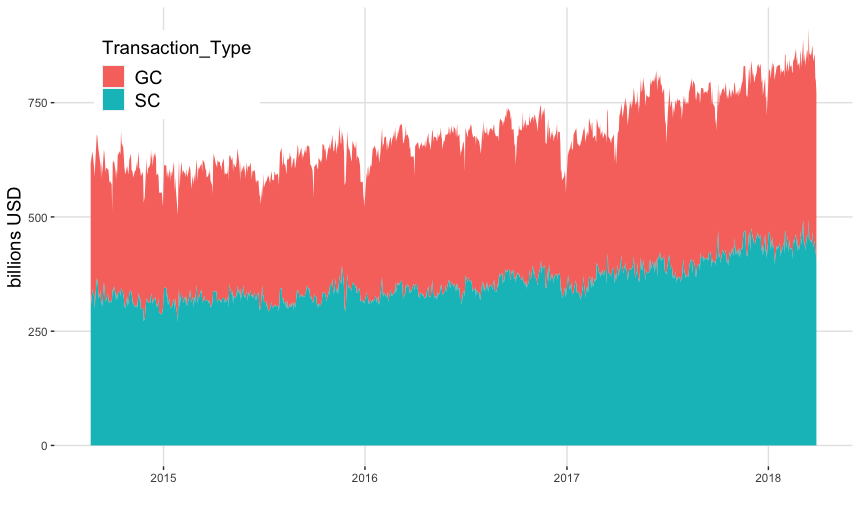
\includegraphics[scale=.5]{fig1.png}
\end{center}


\subsubsection{Treasuries Outstanding and Scarcity Value}
Intuitively,  when the volume of outstanding Treasuries is larger,  the Treasuries as collateral become less scarcity,  so the rate spread between bilateral repo transactions and tri-party repo transactions increases.  

\begin{center}
\begin{tabular}{@{\extracolsep{5pt}}lD{.}{.}{-3} D{.}{.}{-3} } 
\\[-1.8ex]\hline 
\hline \\[-1.8ex] 
 & \multicolumn{2}{c}{\textit{Dependent variable:}} \\ 
\cline{2-3} 
\\[-1.8ex] & \multicolumn{2}{c}{SC repo rate - GC repo rate} \\ 
\\[-1.8ex] & \multicolumn{1}{c}{(1)} & \multicolumn{1}{c}{(2)}\\ 
\hline \\[-1.8ex] 
$\Delta$log treasuries & 1,280.301^{***} & 1,321.397^{***} \\ 
  & (232.948) & (221.020) \\ 
$\Delta$log GC volume &  & -46.675^{***} \\ 
  &  & (4.473) \\ 
$\Delta$log SC volume&  & 6.483 \\ 
  &  & (4.377) \\ 
  Constant & -0.236 & -0.238 \\ 
  & (0.225) & (0.212) \\ 
 \hline \\[-1.8ex] 
Observations & \multicolumn{1}{c}{899} & \multicolumn{1}{c}{899} \\ 
R$^{2}$ & \multicolumn{1}{c}{0.033} & \multicolumn{1}{c}{0.138} \\ 
Adjusted R$^{2}$ & \multicolumn{1}{c}{0.031} & \multicolumn{1}{c}{0.135} \\ 
Residual Std. Error & \multicolumn{1}{c}{6.591 (df = 897)} & \multicolumn{1}{c}{6.230 (df = 895)} \\ 
\hline 
\hline \\[-1.8ex] 
\textit{Note:}  & \multicolumn{2}{r}{$^{*}$p$<$0.1; $^{**}$p$<$0.05; $^{***}$p$<$0.01} \\ 
\end{tabular} 
\end{center}


\newpage
\subsection{Local Projection}
To show that the extra response in SOFR with respect to government borrowing is significantly large and persistent,
I conduct time series analysis using Local Projection with monthly data covering the period
between 2014/08 and 2019/12. In the first stage, I identify the government borrowing shock
using the following strategy:
\begin{align*}
  b_t=\alpha_0+\alpha_1t+\alpha_2t^2+A(L)X_{t-1}+\epsilon_t^b,
\end{align*}
where $b_t$ denotes log(govt debt); $X_t$ denotes controls including six lags of log(govt debt), log(industrial production), and log(stock price)
\footnote{Identifying the government borrowing shock using twelve lags obtains similar result.}; and
$\hat{\epsilon}_t^b$ is adopted as the identified borrowing shock. In the second stage, I estimate the following equation to generate the impulse response functions of SOFR and LIBOR to a standard deviation of government
borrowing shock.
\begin{align*}
  r_{t+h}=\beta_0+\psi_h \hat{\epsilon}_t^b +\Gamma(L)Z_{t-1}+u_{t+h},
\end{align*}
where $r_{t+h}$ denotes SOFR or LIBOR spread at horizon h; $Z_{t-1}$ denotes controls including three lags of SOFR or LIBOR spread, log(govt debt), and log(industrial production).
The IRFs are given in graphs below. Note that SOFR spread exhibits a positive and persistent response to government
borrowing shock for as long as 12 horizons (months) after the shock happens. A simple numerical analysis reveals that a 1-percentage increase in government debt outstanding, which is equivalent to a
0.75-percentage change in GDP \footnote{In dollar value, this is roughly 146 billion.}, results in a 0.8-percentage rise in SOFR right after the borrowing shock. 
This effect remains positive within the following 12 months and peaks at 3.3-percentages in 8 months after the shock.
On the other hand, LIBOR spread responds ambiguously. Two robustness checks are conducted. In the first alternative specification, I replace industrial production with unemployment rate as a measure of output,
the resulting IRFs are very similar. Also, in order to exclude the possible effect from price level, CPI is employed as a control in the second alternative specification, and the results remain unchanged.
\begin{center}
  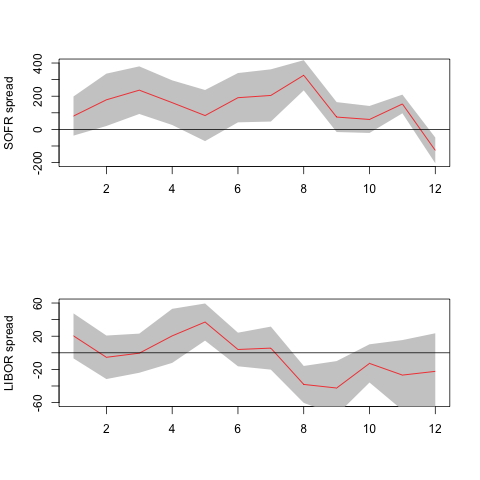
\includegraphics[scale=0.8]{../lp/results/irfs.png}
\end{center}

\newpage
\section{Basic Model}
\subsection{Main Features}
In this section, I model two economies in which firms' borrowing cost is denoted using
SOFR and LIBOR, respectively. The SOFR economy is borrowed from Aiyagari and McGrattan (1998).
The LIBOR economy differs from SOFR economy as banks play a role in providing business 
loans to firms. Under both economies, households choose consumption and saving, while 
providing labor inelastically.












\end{document}

